\chapter{Resultados}
\label{cap:resultados}

\section{Sinal Preditivo}
\label{sec:resultados-skill}

A qualidade do sinal preditivo de cada modelo é medida pelo Rank IC --- correlação de Spearman entre os retornos previstos e os retornos realizados no cross-section de cada data --- e pelo Rank ICIR, que é a razão entre a média e o desvio-padrão do Rank IC ao longo do período de teste. O Rank IC mede a força do sinal de ordenação sem depender da estratégia de portfólio; o ICIR mede sua consistência temporal. Um modelo com IC alto e ICIR baixo produz um sinal que, embora forte em média, oscila entre datas com boa e má capacidade de discriminação. A Tabela~\ref{tab:skill} reporta ambas as métricas para cada modelo.

\begin{table}[htbp]
    \centering
    \caption{Qualidade do sinal preditivo no conjunto de teste.}
    \label{tab:skill}
    \begin{tabular}{lcc}
        \toprule
        \textbf{Modelo}    & \textbf{Rank IC médio} & \textbf{Rank ICIR} \\
        \midrule
        \textbf{FactorVAE} & 0{,}040                & 0{,}246            \\
        GRU                & 0{,}025                & 0{,}217            \\
        IPCA               & 0{,}016                & 0{,}113            \\
        CA                 & 0{,}035                & 0{,}219            \\
        \bottomrule
    \end{tabular}
    \fonte{Elaboração própria.}
\end{table}

O FactorVAE obtém o maior Rank IC (0{,}040), seguido pelo CA (0{,}035), pelo GRU (0{,}025) e pelo IPCA (0{,}016). A mesma ordenação se mantém em Rank ICIR, com o FactorVAE liderando (0{,}246). O CA apresenta ICIR (0{,}219) próximo ao do GRU (0{,}217), apesar de IC superior --- o sinal do CA é, em média, mais forte, mas proporcionalmente mais volátil.

A magnitude da vantagem do FactorVAE sobre o GRU em Rank IC é de 0{,}015 (60\% relativo). Essa diferença é consistente com a contribuição da estrutura fatorial probabilística e do esquema professor-aluno, que são os dois componentes que o FactorVAE adiciona sobre uma GRU pura. A distância para o IPCA (0{,}024 em IC, 150\% relativo) reflete a limitação de um modelo de fatores com exposições lineares em um ambiente onde as relações entre características e retornos são provavelmente não-lineares.

Em comparação com os resultados de \textcite{duan2022} no mercado A-share chinês --- onde o FactorVAE alcança Rank IC de 0{,}055 e ICIR de 0{,}568 ---, os valores obtidos na B3 são menores em magnitude (0{,}040 vs.\ 0{,}055 em IC; 0{,}246 vs.\ 0{,}568 em ICIR). A ordenação qualitativa, porém, se reproduz: o FactorVAE lidera em ambas as métricas sobre os demais modelos de fatores dinâmicos e sobre os baselines de predição. A redução em magnitude é esperada dado o universo substancialmente menor ($\approx$300--500 ativos na B3 vs.\ $>$3.000 no mercado chinês) e a menor liquidez de parte do cross-section brasileiro.


\section{Backtest}
\label{sec:resultados-performance}

O sinal preditivo da seção anterior é traduzido em portfólio pela estratégia TopK-Drop: a cada data, os $k = 50$ ativos com maior retorno previsto ($\mu_y^{(i)}$) compõem uma carteira igual-ponderada, com no máximo $n = 5$ substituições por dia para controlar o giro. Um custo de 25~bps \textit{one-way} é aplicado a cada troca de ativo. A Tabela~\ref{tab:performance} reporta as métricas de performance ajustada ao risco; as Figuras~\ref{fig:retorno-acumulado} e~\ref{fig:retorno-excesso} mostram a trajetória temporal do retorno acumulado absoluto e em excesso sobre o Ibovespa. O Índice de Sharpe é calculado com taxa de referência de 10\% a.a.\ (referência Selic no período).

\begin{table}[htbp]
    \centering
    \caption{Performance ajustada ao risco no período de teste (TopK-Drop, $k=50$, custo 25~bps \textit{one-way}, taxa de referência 10\%~a.a.).}
    \label{tab:performance}
    \resizebox{\textwidth}{!}{%
    \begin{tabular}{lcccccccc}
        \toprule
        \textbf{Modelo}    & \textbf{CAGR}    & \textbf{Ret.\ Acum.} & \textbf{Excesso} & \textbf{Vol.}    & \textbf{Sharpe}  & \textbf{IR}      & \textbf{Calmar}  & \textbf{Max DD}  \\
        \midrule
        \textbf{FactorVAE} & 9{,}97\%         & 97{,}05\%            & $-$0{,}81\%      & 19{,}72\%        & $-$0{,}002       & $-$0{,}028       & 0{,}242          & 41{,}24\%        \\
        Ibovespa           & 10{,}78\%        & 107{,}92\%           & ---              & 23{,}49\%        & 0{,}033          & ---              & 0{,}230          & 46{,}82\%        \\
        GRU                & 6{,}69\%         & 58{,}73\%            & $-$4{,}09\%      & 21{,}96\%        & $-$0{,}151       & $-$0{,}133       & 0{,}139          & 48{,}29\%        \\
        IPCA               & $-$2{,}23\%      & $-$14{,}89\%         & $-$13{,}01\%     & 27{,}24\%        & $-$0{,}449       & $-$0{,}382       & $-$0{,}038       & 58{,}10\%        \\
        CA                 & 6{,}72\%         & 59{,}10\%            & $-$4{,}06\%      & 20{,}54\%        & $-$0{,}160       & $-$0{,}135       & 0{,}150          & 44{,}93\%        \\
        \bottomrule
    \end{tabular}}
    \fonte{Elaboração própria.}
\end{table}

\begin{figure}[htbp]
    \centering
    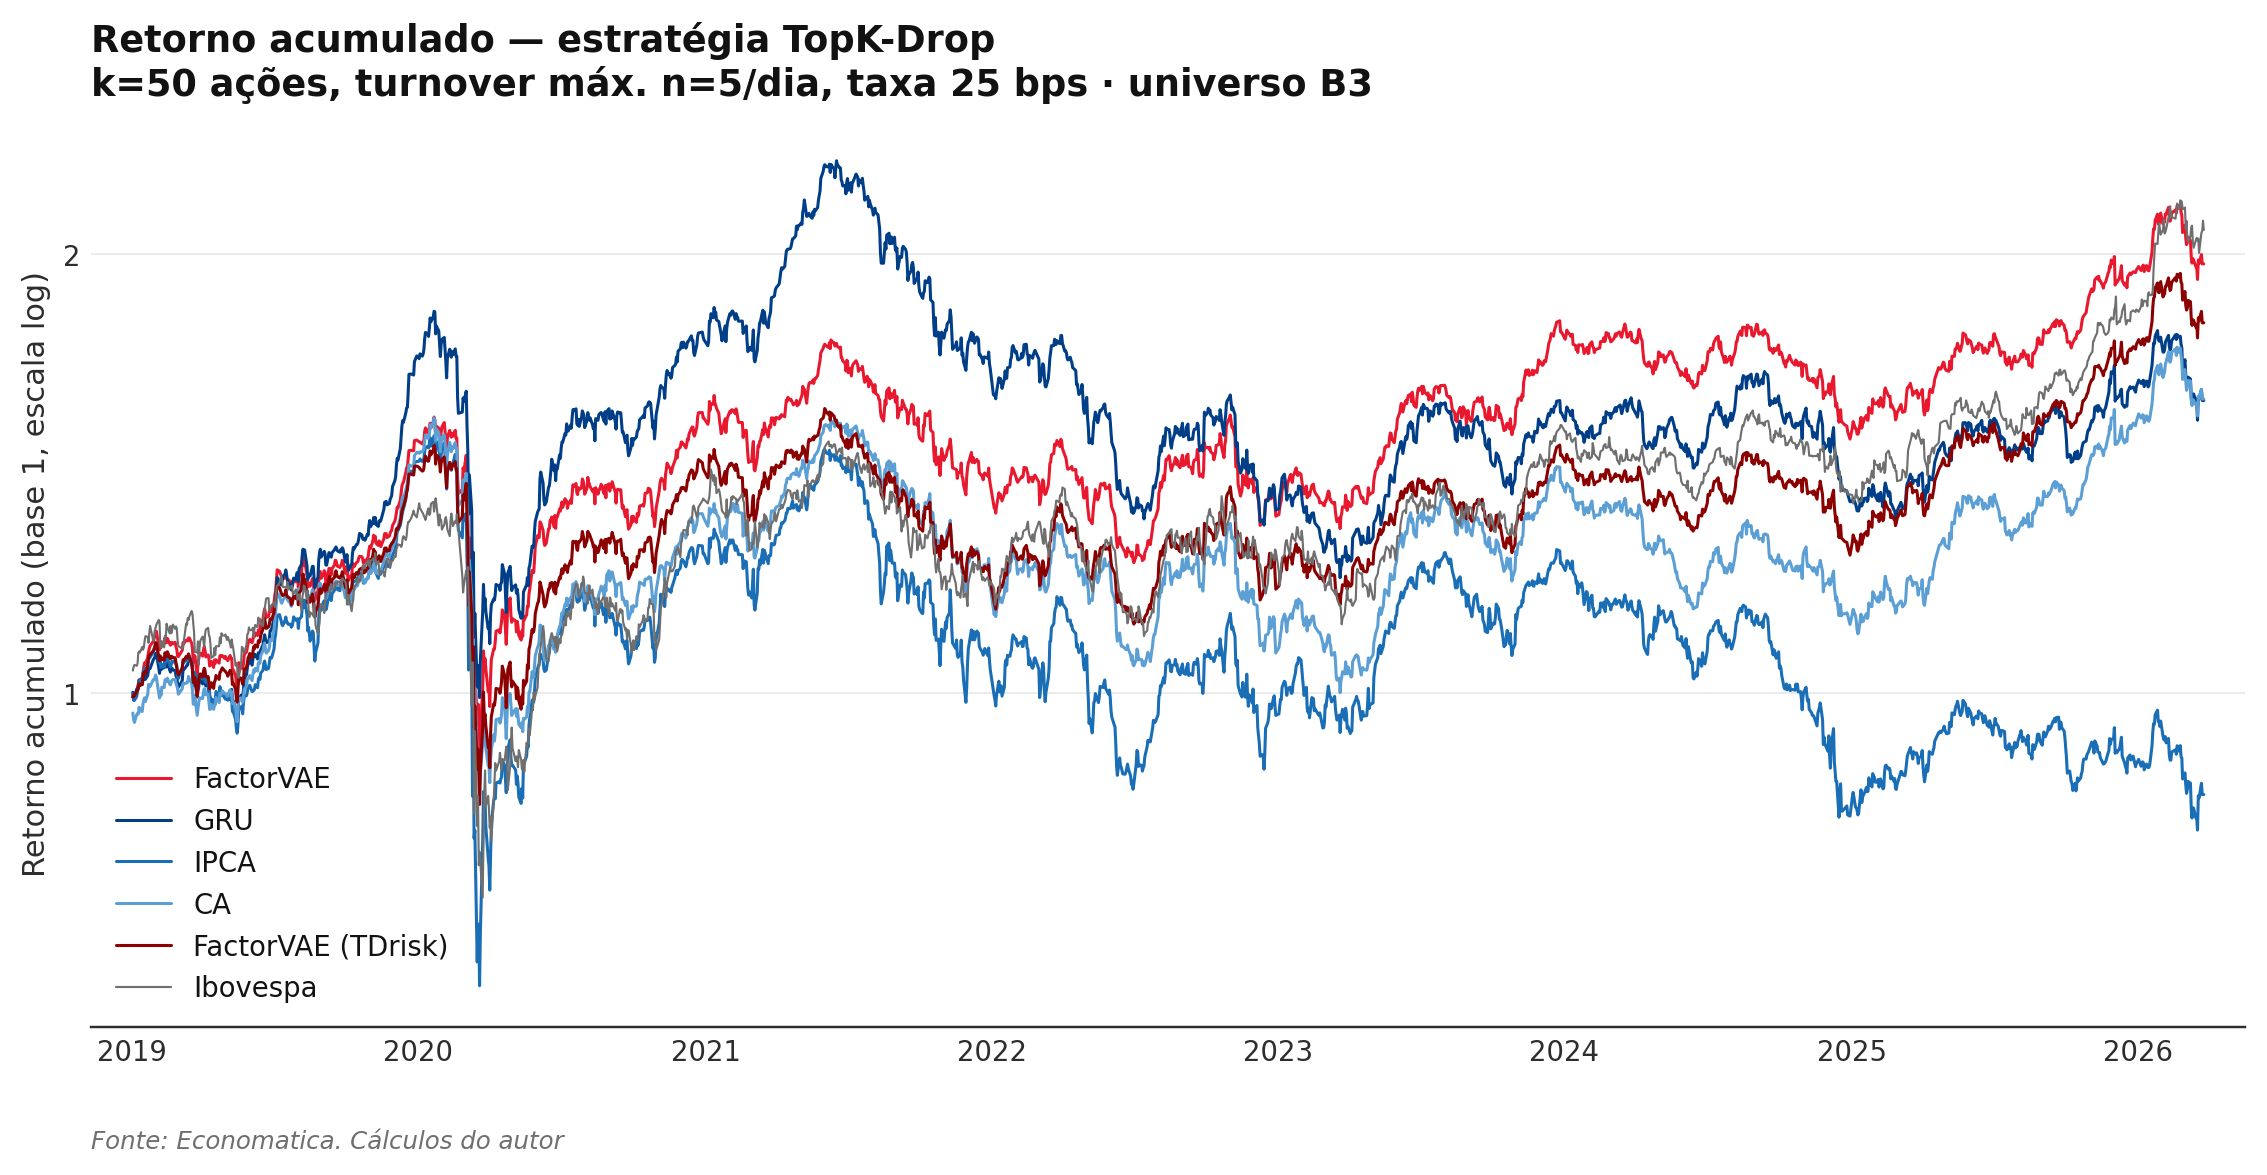
\includegraphics[width=0.95\textwidth]{figuras/BKT_cumulative_return.png}
    \caption{Retorno acumulado da estratégia TopK-Drop por modelo no período de teste.}
    \label{fig:retorno-acumulado}
\end{figure}

\begin{figure}[htbp]
    \centering
    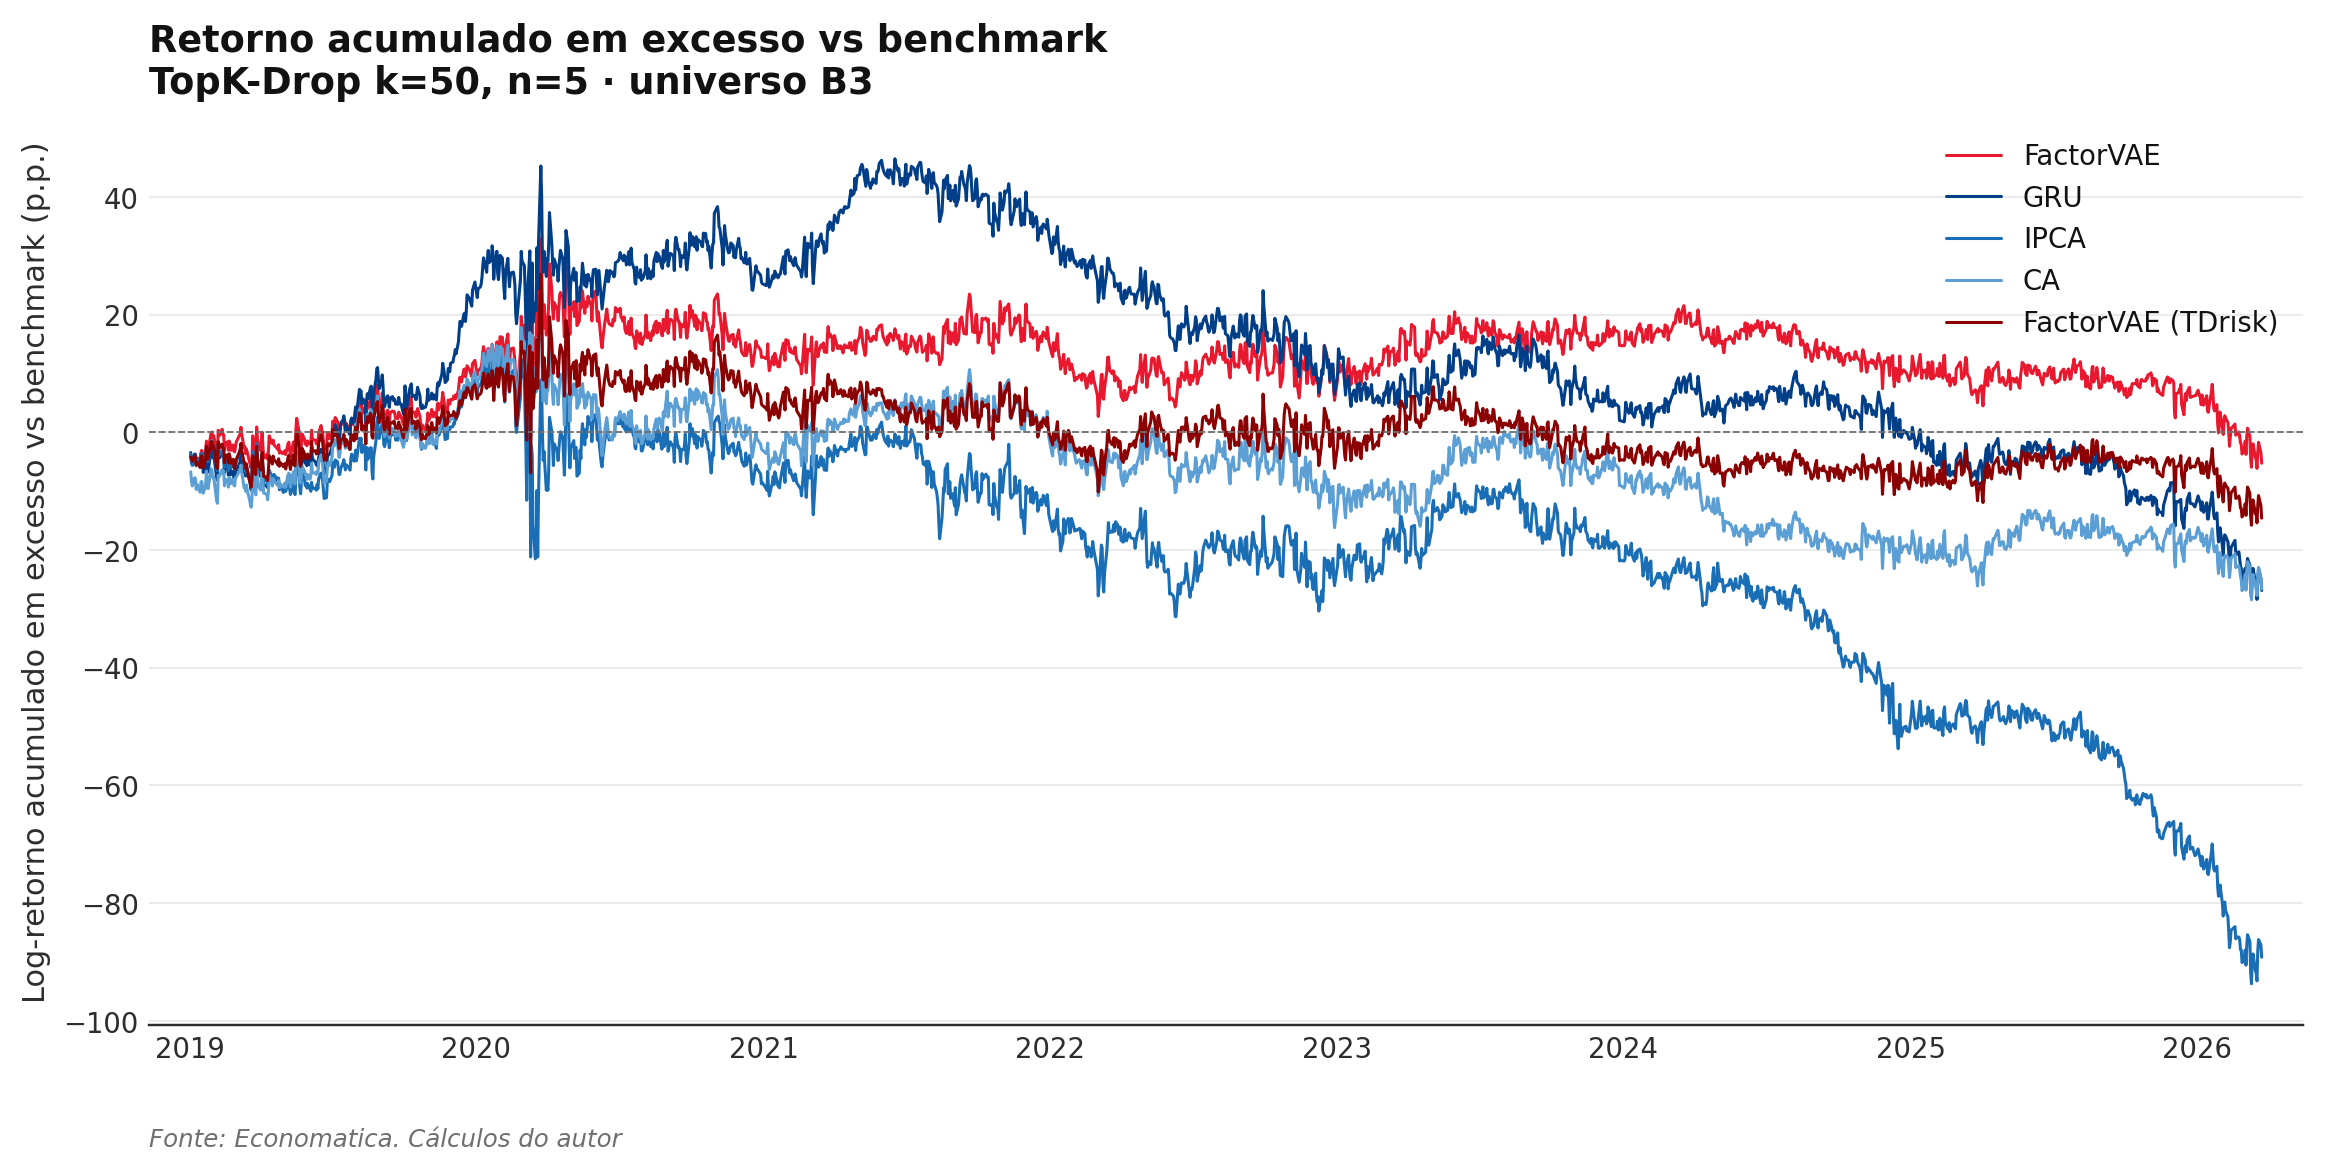
\includegraphics[width=0.95\textwidth]{figuras/BKT_cumulative_excess_return.png}
    \caption{Retorno acumulado em excesso sobre o benchmark.}
    \label{fig:retorno-excesso}
\end{figure}

O FactorVAE apresenta o maior CAGR entre os modelos avaliados (9{,}97\%), seguido pelo CA (6{,}72\%) e pelo GRU (6{,}69\%). A diferença de 3{,}25~p.p.\ anualizados sobre o GRU é economicamente relevante no horizonte do teste (retorno acumulado de 97{,}05\% vs.\ 58{,}73\%). O IPCA é o único modelo com CAGR negativo ($-2{,}23$\%), o que indica que exposições lineares em características não capturam sinal suficiente para compensar os custos de transação neste universo.

O FactorVAE também registra a menor volatilidade anualizada (19{,}72\%) e o menor drawdown máximo (41{,}24\%) entre todos os modelos. Essa combinação de retorno superior e risco inferior resulta em um Sharpe de $-0{,}002$ --- praticamente neutro, dado que o CAGR da estratégia praticamente iguala a taxa de referência. O GRU, com Sharpe de $-0{,}151$, e o CA, com $-0{,}160$, ficam substancialmente abaixo. A Figura~\ref{fig:retorno-acumulado} confirma que a curva do FactorVAE se mantém acima dos demais modelos ao longo de todo o período, com menor amplitude de oscilação.

O resultado central, porém, é que nenhum modelo ativo supera o Ibovespa (CAGR de 10{,}78\%) em retorno absoluto no período observado. A diferença de $-0{,}81$~p.p.\ anualizados entre o FactorVAE e o Ibovespa coexiste com volatilidade 3{,}77~p.p.\ menor (19{,}72\% vs.\ 23{,}49\%) e drawdown 5{,}58~p.p.\ menor (41{,}24\% vs.\ 46{,}82\%). A Figura~\ref{fig:retorno-excesso} mostra que o retorno acumulado em excesso do FactorVAE oscila em torno de zero ao longo do período, sem tendência clara de acumulação positiva ou negativa. O FactorVAE lidera entre os modelos do experimento, mas a vantagem se materializa na dimensão de risco e não na de retorno absoluto.

Essa configuração é consistente com a de \textcite{duan2022} em escala reduzida. No artigo original, o FactorVAE gera alfa positivo sobre o CSI300 com $k = 50$ em um universo de 3.000+ ativos, onde a fração selecionada ($\approx$1{,}5\%) permite maior seletividade. Na B3, $k = 50$ corresponde a $\approx$10--17\% do cross-section, o que dilui mecanicamente o poder de discriminação do sinal e reduz a margem disponível para converter ranking em retorno em excesso.